\documentclass{article}
\usepackage{amsmath, amssymb, amsfonts, bm}
\usepackage{geometry}
\usepackage{tikz}
\usetikzlibrary{arrows.meta}
\usepackage{float}	
\usepackage{graphicx}
\usepackage[colorlinks=true, allcolors=blue]{hyperref}
\usepackage{algorithm}
\usepackage{algpseudocode}
\usepackage{caption}
\usepackage{todo}
\geometry{a4paper, margin=1in}


\begin{document}
	
	\title{Finite Element Formulation of the Extended Euler-Bernoulli Beam with Axial Forces}
	\author{}
	\date{}
	\maketitle
	
	\section*{Governing Equation}
	\section*{Nomenclature}
	\begin{tabular}{p{2cm} p{1cm} p{11cm}}
		$E$           & [Pa]    & Young’s modulus (steel: $2.1\times10^{11}$).\\
		$A$           & [m$^2$] & Cross‐sectional area (e.g. $0.01$).\\
		$I$           & [m$^4$] & Second moment of area (e.g. $8.333\times10^{-6}$).\\
		$\rho$        & [kg/m$^3$]& Mass density (e.g. $7850$).\\
		$L$           & [m]     & Total beam length (e.g. $2$).\\
		$L_e$         & [m]     & Element length: $L_e=L/n_{\mathrm{elem}}$.\\
		$x$           & [m]     & Spatial coordinate.\\
		$t$           & [s]     & Time coordinate.\\
		$u(x,t)$      & [m]     & Axial displacement.\\
		$w(x,t)$      & [m]     & Transverse displacement.\\
		$\delta u,\;\delta w$ & – & Virtual (test) displacements.\\
		$k_e$         & –       & Full element stiffness matrix (6×6).\\
		$m_e$         & –       & Full element mass matrix (6×6).\\
	\end{tabular}
	
	\section{Governing Equations}
	The classical Euler–Bernoulli beam equation for transverse deflection \(w(x,t)\) is
	\begin{equation}\label{eq:transverse_classical}
		EI\,w''''(x,t)
		+\rho A\,\ddot w(x,t)
		= q(x,t).
	\end{equation}
	
	With an added axial degree of freedom, the beam’s strong form separates into two equations:
	\begin{equation}\label{eq:axial_strong}
		\rho A\,\ddot u(x,t)
		- \bigl(EA\,u'(x,t)\bigr)'
		= q(x,t),
	\end{equation}
	\begin{equation}\label{eq:transverse_strong}
		\rho A\,\ddot w(x,t)
		- \bigl(EI\,w''(x,t)\bigr)''
		= q(x,t).
	\end{equation}
	
	An example of beam under analysis is shown in Figure~\ref{fig:FFB}. The beam is fixed at both ends and loaded transversely at its center by a point force \(P\), resulting in internal axial forces \(N_A\), \(N_B\), bending moments \(M_A\), \(M_B\), and vertical reaction forces \(F_A\), \(F_B\).
	\begin{figure}[H]
		\centering
		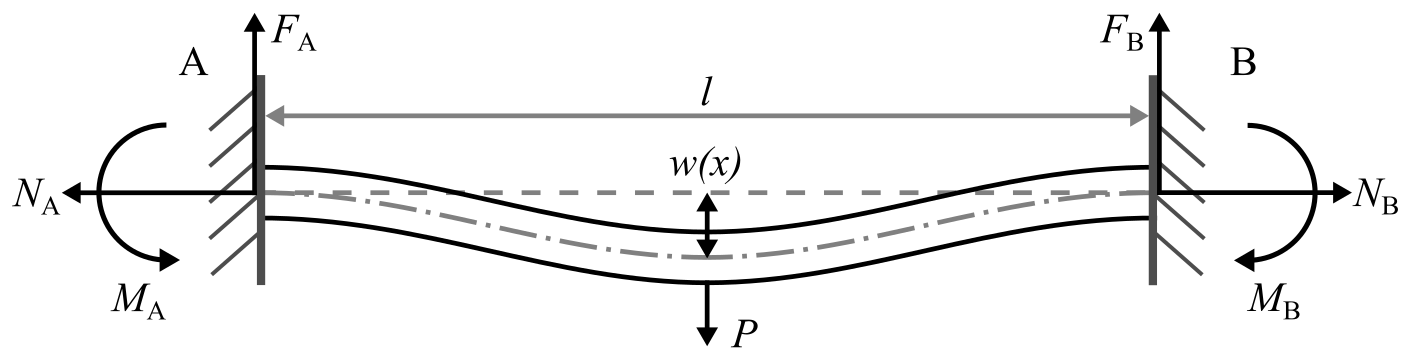
\includegraphics[width=4.7in]{Figures/FFB_Figure.png}
		\caption[FFB]{\label{fig:FFB} 
			Free body diagram of a fixed-fixed beam subjected to a transverse point load.}
	\end{figure} 
	
	\textbf{Explanation for Trotter:} This is the main rule that tells us how the beam bends and moves when a force is applied.
	
	\section{Weak Form}
	To reduce the continuity requirements on trial and test spaces and to impose natural boundary conditions, we derive the variational form by multiplying each strong equation by its virtual displacement and integrating by parts.
	
	\subsection{Axial}
	Multiply Eq.~\eqref{eq:axial_strong} by \(\delta u\), integrate by parts:
	\begin{equation}\label{eq:axial_weak}
		\int_0^L EA\,u'\,\delta u'\,dx 
		- \bigl[EA\,u'\,\delta u\bigr]_0^L = 0
		\;\Longrightarrow\;
		\int_0^L EA\,u'\,\delta u'\,dx = 0.
	\end{equation}
	
	\subsection{Bending}
	Multiply Eq.~\eqref{eq:transverse_strong} by \(\delta w\), integrate by parts twice:
	\begin{equation}\label{eq:bending_weak}
		\int_0^L EI\,w''\,\delta w''\,dx 
		- \bigl[EI\,w''\,\delta w' - (EI\,w'')'\,\delta w\bigr]_0^L = 0
		\;\Longrightarrow\;
		\int_0^L EI\,w''\,\delta w''\,dx = 0.
	\end{equation}
	
	\section{Finite‐Element Interpolations}
	\subsection{Axial (linear)}
	We approximate \(u(x)\) over each element of length \(L_e\) by
	\begin{equation}\label{eq:axial_interp}
		N^{(u)}(x)
		= \begin{pmatrix}1-\tfrac{x}{L_e}\\[4pt]\tfrac{x}{L_e}\end{pmatrix},
		\qquad
		u(x)=\bigl[N^{(u)}(x)\bigr]^\text{T}(u_1,u_2)^\text{T}.
	\end{equation}
	
	\subsection{Transverse (Hermite cubic)}
	To capture bending curvature with \(C^1\) continuity, we use four cubic polynomials: \todo{all of the subscript "e"s should not be italic, they are not a variable, they are a descriptor. }
	\begin{equation}\label{eq:cubic_interp}
		\begin{aligned}
			N_1(x)&=1-3(\tfrac{x}{L_e})^2+2(\tfrac{x}{L_e})^3,\\
			N_2(x)&=x[1-2(\tfrac{x}{L_e})+(\tfrac{x}{L_e})^2],\\
			N_3(x)&=3(\tfrac{x}{L_e})^2-2(\tfrac{x}{L_e})^3,\\
			N_4(x)&=x[-(\tfrac{x}{L_e})+(\tfrac{x}{L_e})^2].
		\end{aligned}
	\end{equation}
	Mapping \(x\to\xi=x/L_e\in[0,1]\) for integration:
	\begin{equation}\label{eq:map_interp}
		\begin{aligned}
			N_1(\xi)&=1-3\xi^2+2\xi^3,\quad
			N_2(\xi)=L_e\,\xi(1-2\xi+\xi^2),\\
			N_3(\xi)&=3\xi^2-2\xi^3,\quad
			N_4(\xi)=L_e\,\xi(-\xi+\xi^2).
		\end{aligned}
	\end{equation}
	
	\section{Element Stiffness Matrices}
	Substituting the above interpolations into the weak forms (\ref{eq:axial_weak})–(\ref{eq:bending_weak}) and evaluating the resulting integrals yields:
	
	\subsection{Axial}
	By inserting \(u(x)\) from \eqref{eq:axial_interp} into \eqref{eq:axial_weak} and noting the constant derivative,
	\begin{equation}\label{eq:ke_axial}
		k_e^{(\mathrm{axial})}
		= \int_0^{L_e}EA\,\frac{dN^{(u)}}{dx}\frac{dN^{(u)}}{dx}^\text{T}dx
		= \frac{EA}{L_e}
		\begin{pmatrix}1 & -1\\ -1 & 1\end{pmatrix}.
	\end{equation}


	\subsection{Bending}
	From the bending weak form \eqref{eq:bending_weak}, define the curvature–shape vector in \(\xi\):
	\begin{equation}\label{eq:B_vector}
		B(\xi)
		= \frac{d^2N^{(w)}}{dx^2}
		= \frac{1}{L_e^2}[6\xi-6,\;3\xi-4,\;-6\xi+6,\;3\xi-2],
	\end{equation}
	then
	\begin{equation}\label{eq:ke_bending}
		k_e^{(\mathrm{bending})}
		= EI\int_0^{L_e}B^\text{T} B\,dx
		= \frac{EI}{L_e^3}
		\begin{pmatrix}
			12 & 6L_e & -12 & 6L_e\\
			6L_e & 4L_e^2 & -6L_e & 2L_e^2\\
			-12 & -6L_e & 12 & -6L_e\\
			6L_e & 2L_e^2 & -6L_e & 4L_e^2
		\end{pmatrix}.
	\end{equation}
	
	\subsection{Assembled stiffness}
	Finally, the full 6×6 element stiffness matrix is
	\begin{equation}\label{eq:ke_assembled}
		k_e
		= \begin{pmatrix}
			k_e^{(\mathrm{axial})} & \mathbf{0}\\
			\mathbf{0}            & k_e^{(\mathrm{bending})}
		\end{pmatrix}.
	\end{equation}
	
	\section{Element Mass Matrices}
	The element mass matrix comes from the beam’s kinetic energy:
	\begin{equation}
		T
		= \tfrac12\int_0^{L_e}\rho A\,\dot u^2(x,t)\,dx
		+\tfrac12\int_0^{L_e}\rho A\,\dot w^2(x,t)\,dx.
	\end{equation}
	
	\subsection{Axial}
	We start with the axial kinetic energy
	\begin{equation}
		T_{\mathrm{axial}}
		= \tfrac12\int_0^{L_e}\rho A\,\dot u^2\,dx.
	\end{equation}
	Substitute the linear interpolation \eqref{eq:axial_interp}:
	\begin{equation}
		\dot u(x,t)
		= \bigl[N^{(u)}(x)\bigr]^\text{T}\,\dot{\mathbf{u}},
	\end{equation}
	which gives
	\begin{equation}
		T_{\mathrm{axial}}
		= \tfrac12\,\dot{\mathbf{u}}^\text{T}
		\Bigl[\int_0^{L_e}\rho A\,N^{(u)}N^{(u)T}\,dx\Bigr]
		\,\dot{\mathbf{u}}
		= \tfrac12\,\dot{\mathbf{u}}^\text{T}\,m_e^{(\mathrm{axial})}\,\dot{\mathbf{u}}.
	\end{equation}
	Hence the consistent axial mass block is
	\begin{equation}\label{eq:me_axial}
		m_e^{(\mathrm{axial})}
		= \int_0^{L_e}\rho A\,N^{(u)}N^{(u)T}\,dx
		= \frac{\rho A L_e}{6}
		\begin{pmatrix}2 & 1\\ 1 & 2\end{pmatrix}.
	\end{equation}
	
	\subsection{Bending}
	Likewise, for bending
	\begin{equation}
		T_{\mathrm{bend}}
		= \tfrac12\int_0^{L_e}\rho A\,\dot w^2\,dx.
	\end{equation}
	Using the Hermite‐cubic interpolation \eqref{eq:cubic_interp}:
	\begin{equation}
		\dot w(x,t)
		= \bigl[N^{(w)}(\xi)\bigr]^\text{T}\,\dot{\mathbf{w}},
	\end{equation}
	we obtain
	\begin{equation}
		T_{\mathrm{bend}}
		= \tfrac12\,\dot{\mathbf{w}}^\text{T}
		\Bigl[\int_0^{L_e}\rho A\,N^{(w)}(\xi)N^{(w)T}(\xi)\,dx\Bigr]
		\,\dot{\mathbf{w}}
		= \tfrac12\,\dot{\mathbf{w}}^\text{T}\,m_e^{(\mathrm{bending})}\,\dot{\mathbf{w}}.
	\end{equation}
	Thus the bending mass block is
	\begin{equation}\label{eq:me_bending}
		m_e^{(\mathrm{bending})}
		= \int_0^{L_e}\rho A\,N^{(w)}(\xi)N^{(w)T}(\xi)\,dx
		= \frac{\rho A L_e}{420}
		\begin{pmatrix}
			156 & 22L_e & 54 & -13L_e\\
			22L_e & 4L_e^2 & 13L_e & -3L_e^2\\
			54 & 13L_e & 156 & -22L_e\\
			-13L_e & -3L_e^2 & -22L_e & 4L_e^2
		\end{pmatrix}.
	\end{equation}
	
	\subsection{Assembled Mass}
	Putting axial and bending together gives the full element mass matrix:
	\begin{equation}\label{eq:me_assembled}
		m_e
		= \begin{pmatrix}
			m_e^{(\mathrm{axial})} & \mathbf{0}\\
			\mathbf{0}            & m_e^{(\mathrm{bending})}
		\end{pmatrix}.
	\end{equation}
	
	\section{Equation of Motion and Time Integration}
	
	% -------------------------------------------------------------------
	% Before the equation: introduce and define all terms
	% -------------------------------------------------------------------
	The global equation of motion for the discretized beam—assembled from all element mass, damping, and stiffness contributions—can be written in matrix form as
	
	\begin{equation}\label{eq:global_expanded}
		\underbrace{\begin{bmatrix}
				m_{11} & m_{12} & \cdots & m_{1n}\\
				m_{21} & m_{22} & \cdots & m_{2n}\\
				\vdots & \vdots & \ddots & \vdots\\
				m_{n1} & m_{n2} & \cdots & m_{nn}
		\end{bmatrix}}_{M}
		\,
		\underbrace{\begin{bmatrix}
				\ddot u_1\\[4pt]
				\ddot w_1\\[4pt]
				\ddot \theta_1 \\[2pt]
				\vdots \\[2pt]
				\ddot \theta_N
		\end{bmatrix}}_{\ddot W}
		\;+\;
		\underbrace{\begin{bmatrix}
				c_{11} & c_{12} & \cdots & c_{1n}\\
				c_{21} & c_{22} & \cdots & c_{2n}\\
				\vdots & \vdots & \ddots & \vdots\\
				c_{n1} & c_{n2} & \cdots & c_{nn}
		\end{bmatrix}}_{C}
		\,
		\underbrace{\begin{bmatrix}
				\dot u_1\\[4pt]
				\dot w_1\\[4pt]
				\dot \theta_1 \\[2pt]
				\vdots \\[2pt]
				\dot \theta_N
		\end{bmatrix}}_{\dot W}
		\;+\;
		\underbrace{\begin{bmatrix}
				k_{11} & k_{12} & \cdots & k_{1n}\\
				k_{21} & k_{22} & \cdots & k_{2n}\\
				\vdots & \vdots & \ddots & \vdots\\
				k_{n1} & k_{n2} & \cdots & k_{nn}
		\end{bmatrix}}_{K}
		\,
		\underbrace{\begin{bmatrix}
				u_1\\[4pt]
				w_1\\[4pt]
				\theta_1 \\[2pt]
				\vdots \\[2pt]
				\theta_N
		\end{bmatrix}}_{W}
		=
		\underbrace{\begin{bmatrix}
				F_1(t)\\[4pt]
				F_2(t)\\[4pt]
				F_3(t) \\[2pt]
				\vdots \\[2pt]
				F_n(t)
		\end{bmatrix}}_{F(t)}.
	\end{equation}
	
	% -------------------------------------------------------------------
	% After the equation: detailed description of each quantity
	% -------------------------------------------------------------------
	Here:
	\begin{itemize}
		\item \(W = [\,u_1,\;w_1,\;\theta_1,\;\dots,\;u_N,\;w_N,\;\theta_N\,]^\text{T}\) collects all \(3N\) nodal degrees of freedom: 
		\(u_i\) (axial displacement), \(w_i\) (transverse displacement), and \(\theta_i\) (slope) at node \(i\).
		\item \(\ddot W\) and \(\dot W\) are the corresponding acceleration and velocity vectors.
		\item \(M = [m_{ij}]\) is the global mass matrix, assembled from each element’s consistent mass blocks (Eqs.~\eqref{eq:me_axial} and \eqref{eq:me_bending}).
		\item \(C = [c_{ij}]\) is the global damping matrix (e.g.\ Rayleigh damping \(C=\alpha M + \beta K\)).
		\item \(K = [k_{ij}]\) is the global stiffness matrix, assembled from each element’s axial and bending stiffness (Eqs.~\eqref{eq:ke_axial}–\eqref{eq:ke_bending}).
		\item \(F(t) = [F_1(t),F_2(t),\dots,F_n(t)]^\text{T}\) is the vector of external (or control) forces and moments applied at each DOF.
	\end{itemize}
	
	Equation~\eqref{eq:global_expanded} succinctly represents the dynamic equilibrium of the entire beam structure in its finite‐element discretization.
	
		
%%%%%%%%%%%%%%%%%%%%%%%%%%%%%%%%%%%%%%%%%%%%%%%%%%%%%%%%%%%%%%%%%%%%%%%%%%%	

%%% Beginning of the time integration section%%%%%%%%%
	
	\subsection{Dynamic time integration}

	The Newmark--Beta method is a widely used implicit time integration scheme for solving second-order systems of the form:
	\begin{equation}
		\mathit{\mathbf{M}}\, \ddot{\mathit{\mathbf{w}}} + \mathit{\mathbf{C}}\, \dot{\mathit{\mathbf{w}}} + \mathit{\mathbf{K}}\, \mathit{\mathbf{w}} = \mathit{\mathbf{f}}(t),
	\end{equation}
	where \( \mathit{\mathbf{w}}, \dot{\mathit{\mathbf{w}}}, \ddot{\mathit{\mathbf{w}}} \) denote displacement, velocity, and acceleration vectors. The matrices \( \mathit{\mathbf{M}}, \mathit{\mathbf{C}}, \mathit{\mathbf{K}} \) are the mass, damping, and stiffness matrices. The damping matrix is often modeled using Rayleigh damping.
	
	\subsubsection{Determination of Rayleigh Damping Coefficients}
	\todo{does this need to be in the dynamic time integration section?}
	Rayleigh damping is modeled by a linear combination of the mass and stiffness matrices:
	\begin{equation}
		\mathbf{C} = \alpha_R \mathbf{M} + \beta_R \mathbf{K},
	\end{equation}
	where \( \alpha_R \) and \( \beta_R \) are the mass- and stiffness-proportional damping coefficients, respectively.
	
	To determine \( \alpha_R \) and \( \beta_R \), we specify the desired damping ratios \( \zeta_1 \) and \( \zeta_2 \) for two selected natural modes with angular frequencies \( \omega_1 \) and \( \omega_2 \). The damping ratio for each mode is defined as:
	\begin{equation}
		\zeta_i = \frac{\alpha_R}{2\omega_i} + \frac{\beta_R \omega_i}{2}, \quad i = 1, 2.
	\end{equation}
	
	This yields the following system of linear equations:
	\[
	\begin{cases}
		\zeta_1 = \dfrac{\alpha_R}{2\omega_1} + \dfrac{\beta_R \omega_1}{2}, \\\\
		\zeta_2 = \dfrac{\alpha_R}{2\omega_2} + \dfrac{\beta_R \omega_2}{2}.
	\end{cases}
	\]
	
	This system can be rewritten in matrix form:
	\begin{equation}
		\begin{bmatrix}
			\dfrac{1}{2\omega_1} & \dfrac{\omega_1}{2} \\\\
			\dfrac{1}{2\omega_2} & \dfrac{\omega_2}{2}
		\end{bmatrix}
		\begin{bmatrix}
			\alpha_R \\\\
			\beta_R
		\end{bmatrix}
		=
		\begin{bmatrix}
			\zeta_1 \\\\
			\zeta_2
		\end{bmatrix}.
	\end{equation}
	
	Let this system be denoted as \( \mathbf{A} \boldsymbol{x} = \boldsymbol{b} \), where:
	\[
	\mathbf{A} =
	\begin{bmatrix}
		\dfrac{1}{2\omega_1} & \dfrac{\omega_1}{2} \\\\
		\dfrac{1}{2\omega_2} & \dfrac{\omega_2}{2}
	\end{bmatrix},
	\quad
	\boldsymbol{x} =
	\begin{bmatrix}
		\alpha_R \\\\
		\beta_R
	\end{bmatrix},
	\quad
	\boldsymbol{b} =
	\begin{bmatrix}
		\zeta_1 \\\\
		\zeta_2
	\end{bmatrix}.
	\]
	
	The damping coefficients are obtained by solving:
	\begin{equation}
		\begin{bmatrix}
			\alpha_R \\\\
			\beta_R
		\end{bmatrix}
		=
		\mathbf{A}^{-1} \boldsymbol{b}.
	\end{equation}
	
	This procedure ensures that the resulting damping matrix \( \mathbf{C} \) produces the desired damping ratios at the specified frequencies. The coefficient \( \alpha_R \) primarily affects low-frequency (inertial) damping, while \( \beta_R \) dominates in high-frequency (stiffness-driven) modes.
	
	
%%%%%%%%%%%%%%%%%%%%%%%%%%%%%%%	
\subsubsection{The implicit time integration}
	At each time step, the Newmark--Beta scheme computes the unknown displacement \( \mathit{\mathbf{w}}_{n+1} \), then updates acceleration and velocity using known values from the previous step. The method uses the following interpolation formulas:
	\begin{align}
		\mathit{\mathbf{w}}_{n+1} &= \mathit{\mathbf{w}}_n + \Delta t\, \dot{\mathit{\mathbf{w}}}_n + \frac{1}{2} \Delta t^2 \left[ (1 - 2\beta) \ddot{\mathit{\mathbf{w}}}_n + 2\beta \ddot{\mathit{\mathbf{w}}}_{n+1} \right], \\
		\dot{\mathit{\mathbf{w}}}_{n+1} &= \dot{\mathit{\mathbf{w}}}_n + \Delta t \left[ (1 - \gamma) \ddot{\mathit{\mathbf{w}}}_n + \gamma \ddot{\mathit{\mathbf{w}}}_{n+1} \right],
	\end{align}
	where \( \beta \) and \( \gamma \) are method parameters. The common choice \( \beta = \tfrac{1}{4} \), \( \gamma = \tfrac{1}{2} \) gives unconditional stability and second-order accuracy.
	
	To initiate the time integration, the initial acceleration is computed using:
	\begin{equation}
		\ddot{\mathit{\mathbf{w}}}_0 = \mathit{\mathbf{M}}^{-1} \left[ \mathit{\mathbf{f}}_0 - \mathit{\mathbf{C}}\, \dot{\mathit{\mathbf{w}}}_0 - \mathit{\mathbf{K}}\, \mathit{\mathbf{w}}_0 \right].
	\end{equation}
	
	The effective stiffness matrix is defined by:
	\begin{equation}
		\mathit{\mathbf{K}}_{\text{eff}} = \mathit{\mathbf{K}} + \frac{\gamma}{\beta \Delta t} \mathit{\mathbf{C}} + \frac{1}{\beta \Delta t^2} \mathit{\mathbf{M}}.
	\end{equation}
	
	The effective force vector is assembled from known values:
	\begin{align}
		\mathit{\mathbf{F}}_{\text{eff}} = \mathit{\mathbf{f}}_{n+1}
		&+ \mathit{\mathbf{M}} \left( \frac{1}{\beta \Delta t^2} \mathit{\mathbf{w}}_n + \frac{1}{\beta \Delta t} \dot{\mathit{\mathbf{w}}}_n + \frac{1 - 2\beta}{2\beta} \ddot{\mathit{\mathbf{w}}}_n \right) \\
		&+ \mathit{\mathbf{C}} \left( \frac{\gamma}{\beta \Delta t} \mathit{\mathbf{w}}_n + \left( \frac{\gamma}{\beta} - 1 \right) \dot{\mathit{\mathbf{w}}}_n + \Delta t \left( \frac{\gamma}{2\beta} - 1 \right) \ddot{\mathit{\mathbf{w}}}_n \right).
	\end{align}
	
	The displacement is computed by solving:
	\begin{equation}
		\mathit{\mathbf{K}}_{\text{eff}}\, \mathit{\mathbf{w}}_{n+1} = \mathit{\mathbf{F}}_{\text{eff}}.
	\end{equation}
	
	The acceleration and velocity at the new time step are updated as:
	\begin{align}
		\ddot{\mathit{\mathbf{w}}}_{n+1} &= \frac{1}{\beta \Delta t^2} \left( \mathit{\mathbf{w}}_{n+1} - \mathit{\mathbf{w}}_n - \Delta t \dot{\mathit{\mathbf{w}}}_n \right) - \frac{1 - 2\beta}{2\beta} \ddot{\mathit{\mathbf{w}}}_n, \\
		\dot{\mathit{\mathbf{w}}}_{n+1} &= \dot{\mathit{\mathbf{w}}}_n + \Delta t \left[ (1 - \gamma) \ddot{\mathit{\mathbf{w}}}_n + \gamma \ddot{\mathit{\mathbf{w}}}_{n+1} \right].
	\end{align}
	
	The influence of Rayleigh damping is embedded directly in the matrix solve. The coefficient \( \alpha_R \) provides damping for lower-frequency (mass-dominated) modes, while \( \beta_R \) suppresses higher-frequency (stiffness-dominated) vibrations. This results in a stable and physically realistic solution, particularly in systems with broad frequency content.
	
	
%%%%%%%%%%%%%%%%%%%%%%%%%%%%%%	
	\subsubsection{Central Difference Explicit Time Integration}
	
	The central difference method is a second-order explicit time integration technique suitable for wave propagation and dynamic response problems. The update of displacement is given by:
	\begin{equation}
		\mathbf{w}_{n+1} = \Delta t^2 \mathbf{M}^{-1} \left[ \mathbf{f}_n - \mathbf{K} \mathbf{w}_n - \mathbf{C} \left( \frac{\mathbf{w}_n - \mathbf{w}_{n-1}}{\Delta t} \right) \right] + 2\mathbf{w}_n - \mathbf{w}_{n-1},
	\end{equation}
	where \( \mathbf{C} = \alpha_R \mathbf{M} + \beta_R \mathbf{K} \) is the Rayleigh damping matrix. This formulation includes both stiffness and mass proportional damping contributions.
	
	We proceed as follows:
	

	Assume initial displacement \( \mathbf{w}_0 \), and velocity \( \dot{\mathbf{w}}_0 \). Compute the initial acceleration from the equation of motion:
	\begin{equation}
		\ddot{\mathbf{w}}_0 = \mathbf{M}^{-1} \left( \mathbf{f}_0 - \mathbf{C} \dot{\mathbf{w}}_0 - \mathbf{K} \mathbf{w}_0 \right).
	\end{equation}
	
Using a Taylor expansion for a special start (explicit scheme has no \( \mathbf{w}_{-1} \)):
	\begin{equation}
		\mathbf{w}_1 = \mathbf{w}_0 + \Delta t \dot{\mathbf{w}}_0 + \frac{1}{2} \Delta t^2 \ddot{\mathbf{w}}_0.
	\end{equation}
	If \( \dot{\mathbf{w}}_0 = 0 \), this simplifies to:
	\begin{equation}
		\mathbf{w}_1 = \mathbf{w}_0 + \frac{1}{2} \Delta t^2 \ddot{\mathbf{w}}_0.
	\end{equation}
	
For \( n \geq 1 \), we use the central difference recurrence:
	\begin{equation}
		\mathbf{w}_{n+1} = \Delta t^2 \mathbf{M}^{-1} \left[ \mathbf{f}_n - \mathbf{K} \mathbf{w}_n - \mathbf{C} \left( \frac{\mathbf{w}_n - \mathbf{w}_{n-1}}{\Delta t} \right) \right] + 2\mathbf{w}_n - \mathbf{w}_{n-1}.
	\end{equation}
	
Velocity and acceleration can be recovered at each time step using finite differences:
	\begin{align}
		\dot{\mathbf{w}}_n &= \frac{\mathbf{w}_{n+1} - \mathbf{w}_{n-1}}{2\Delta t}, \\
		\ddot{\mathbf{w}}_n &= \frac{\mathbf{w}_{n+1} - 2\mathbf{w}_n + \mathbf{w}_{n-1}}{\Delta t^2}.
	\end{align}
	
	
	It is important to note that explicit time integration methods are conditionally stable and require careful selection of the time step to maintain numerical stability. The stability criterion is typically governed by the following inequality:
	:
	
	\begin{equation}
		\Delta t < \frac{2}{\omega_{\max}},
	\end{equation}
	
	where \( \omega_{\max} \) represents the highest natural frequency of the system. This value is directly associated with the largest eigenvalue of the matrix \( \mathbf{M}^{-1} \mathbf{K} \), where \( \mathbf{M} \) and \( \mathbf{K} \) are the global mass and stiffness matrices, respectively. If this condition is not met, the numerical solution may become unstable and diverge.
	
	
%	\subsubsection{Explicit vs. Implicit Time Integration: Trade-offs and Applications}
%	
%	Time integration schemes in structural dynamics can broadly be classified into explicit and implicit methods, each offering distinct advantages and limitations. Explicit methods, such as the central difference scheme, compute the system's state at the next time step using only previously known values. As a result, they do not require the solution of a global system of equations at each time step, making them computationally attractive for large-scale problems with sparse matrices. This efficiency becomes particularly valuable when dealing with high-resolution finite element models where direct or iterative solvers for implicit schemes would be prohibitively expensive.
%	
%	However, explicit schemes are conditionally stable and require careful selection of a time step that satisfies a critical stability condition, typically dictated by the maximum natural frequency of the system. This limitation often necessitates the use of extremely small time steps, especially in stiff systems, which can result in high computational cost for long-duration simulations. Despite this, explicit methods are highly effective for problems dominated by short-duration, high-speed transients—such as impact loading, wave propagation, and shock dynamics—where the small time step aligns naturally with the physics of the problem.
%	
%	In contrast, implicit methods, such as the Newmark--Beta scheme with appropriate parameters, are unconditionally stable for linear problems and allow larger time steps without compromising numerical stability. However, this comes at the cost of solving a linear or nonlinear system of equations at every time step, which can be computationally demanding for large systems. Furthermore, implicit methods tend to damp out high-frequency modes unless specifically accounted for, making them less suitable for capturing sharp transients or high-frequency responses.
%	
%	In summary, the choice between explicit and implicit time integration depends on the problem characteristics. Explicit methods are preferred when dealing with large, sparse systems subject to high-speed, short-duration dynamics where accurate tracking of high-frequency content is essential. Implicit methods, on the other hand, are better suited for problems involving slower dynamics or those requiring long time simulations with moderate accuracy and stability demands.
	
	
	
	
%%%%%%%%%%%%%%%%%%%%%%%%%%%%%%%%%%%%%%%%%%%%%%%%%%%%%%%%%%%%%%%%%%%%%%%%%	
	
	
	
	
	
	
	\section*{Control Force Calculation}
	Control forces are introduced at selected nodes along the beam to actively influence both axial and bending responses. As shown in Figure~\ref{fig:control_forces}, each actuator applies a concentrated axial force \( F_{\text{control}} \) along the beam axis and induces a moment \( M_{\text{control}} \) by acting off-center relative to the beam’s neutral axis. These control actions are designed to counteract undesirable vibrations or deflections and are computed based on real-time deviations from a desired trajectory or shape.
	
	The control force is defined as
	\begin{equation}
		F_{\text{control}} = K_{\text{ctrl}} \cdot e(t),
	\end{equation}
	where \( K_{\text{ctrl}} \) represents a control gain and \( e(t) \) is the error between the measured and desired beam states. The corresponding moment is defined as
	\begin{equation}
		M_{\text{control}} = F_{\text{control}} \cdot \frac{h}{2},
	\end{equation}
	where \( h \) is the beam thickness, and the factor \( h/2 \) accounts for the distance from the neutral axis to the surface where the actuator applies the force.
	
	In the finite element framework, \( F_{\text{control}} \) is applied to the axial degree of freedom \( u \) at the control node, while \( M_{\text{control}} \) contributes to the rotational degree of freedom \( \theta \) at the same node. These contributions are inserted directly into the global force vector in the positions corresponding to those degrees of freedom.
	
	The modified equation of motion, including the control forces and moments, becomes
	\begin{equation}
		M \ddot{W} + C \dot{W} + K W = F_{\text{control}}(t),
	\end{equation}
	where \( M \), \( C \), and \( K \) are the assembled global mass, damping, and stiffness matrices, and \( F_{\text{control}}(t) \) contains the time-varying control inputs mapped to the appropriate DOFs.
	
	\begin{figure}[H]
		\centering
		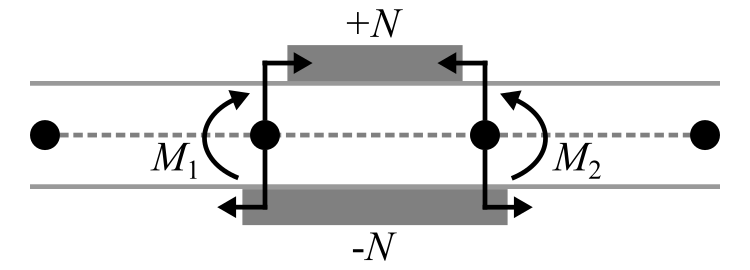
\includegraphics[width=2.4in]{Figures/ControlForces_Figure.png}
		\caption{Control force \( F_{\text{control}} \) and generated moment \( M_{\text{control}} \) applied at the control node.}
		\label{fig:control_forces}
	\end{figure}
	
	\textbf{Explanation for Trotter:} The control force is calculated based on how much the beam is off from where you want it to be. This force is applied at a specific point on the beam, called the control node. Along with this force, a moment is created to control bending. Both are included in the beam’s equations of motion to guide its behavior.
	
\end{document}
